%-------------------------------------------------------------------------------
%	CAPITOLO 35
%-------------------------------------------------------------------------------

\chapter{La festa da ballo dei contadini}
I signori del paese erano rimasti in pochi, vecchi e con grattacapi di cambiali in iscadenza, gli artigiani non valeva altro che poco numericamente, e così il carnevale languiva. \\
\indent L'agricoltura faceva progressi, i contadini cominciavano a star bene, alla galozza (berretto giallo di stoppa) cominciavano a sostituire il cappello, erano molli, affiatati, ubbidienti e disciplinati ai loro capi \index[Personaggi]{Sitì}Sitì, \index[Personaggi]{Gallamini Giovanni `Minten'}Minten\footnote{\textbf{Giovanni Gallamini} (22/12/1865 - 20/05/1944)}, \index[Personaggi]{Piteda}Piteda, \index[Personaggi]{Stuanen}Stuanen ecc.\\
\indent In circa un centinaio, per lo più scapoli, si erano uniti in società, pagavano 20 centesimi a testa ogni domenica, per godersi, o faticare per dare una festa da ballo alla sera della domenica grassa. \\
\indent Le adunanze erano molte, per preparare la gran festa, ricordo che una volta ero in casa \index[Personaggi]{Faggioli}Faggioli e tra una Signorina e Sitì si svolse questo colloquio:\\
\indent La signorina, che era in vena di ridere e far ridere: <<Come devono essere vestite le vostre ballerine?>>\\
\indent Sitì: <<Devono essere vestite di bianco, con nastri e sbraciolate fin qui>> e nel dir ciò indicò l'omero del braccio... ed il discorso seguitò col resto degli spropositi e... stuzzicanti domande.\\
\indent Finalmente siamo alla gran sera, gli inviti a stampa ed aggiunte verbali per le belle ragazze e loro madri erano stati fatti. Alla sera alle 19 precise le ballerine dovevano trovarsi tutte accompagnate dalle loro madri all'osteria. Lì le madri levavano fazzoletti, scialle alle loro figlie, che rimanevano coi finissimi vestiti di raso o seta, e venivano consegnati ai complimentari (quelli incaricati delle cerimonie e che le mettevano in ballo poi) irregimentate, ed al braccio ciascuna a un complimentario, al via del capo sala, marciavano in coppie attraverso la piazza, anche se faceva freddo, pioveva ecc. ed entravano in file nel \index[Luoghi]{Teatro Camerani}Teatro Vecchio\footnote{\textbf{Teatro Camerani}, fu costruito probabilmente nei primi dell'800 da \index[Personaggi]{Camerani dott. Giannantonio (governatore)}Giovannantonio Camerani, avvocato e Giudice di Pace, figlio di \index[Personaggi]{Camerani Matteo (fattore)}Matteo Camerani, fattore della famiglia Spreti che aveva sposato la sorella di Vincenzo Monti, \index[Personaggi]{Monti Maria Cristina}Maria Cristina.}, o \index[Luoghi]{Teatro Calderoni, Baraccone}Baraccone\footnote{\textbf{Teatro Calderoni}, detto `e baracò' fu il terzo teatro dell'800 e del '900 alfonsinese. Un possidente terriero e uomo di spicco in paese \index[Personaggi]{Gessi Eugenio (possidente)}Eugenio Gessi, in società con \index[Personaggi]{Santoni Sebastiano}Sebastiano Santoni, decise di costruire un teatro-cinematografo, tra i primi a nascere in Romagna, un primato per Alfonsine. Lo fece costruire tutto in legno da un falegname di nome \index[Personaggi]{Calderoni Antonio (falegname)}Antonio Calderoni, e la gente lo chiamò amichevolmente `e baracò', il baraccone.} dopo, accolte trionfalmente da un ballabile e dai ballerini.\\
\indent Le madri seguivano le figlie col fagotto degli indumenti che andavano a depositare nel camerino delle ragazze. Le ballerine erano subito messe in ballo, e le loro madri in un cantone a fare da spettatrici e commentare...\\
\indent Alla fine di ogni ballo, vi era il "compermesso" cambio dei ballerini. Questi seguivano le ballerine adocchiate durante gli ultimi giri di ogni ballabile con una mano alzata sulla spalla della ballerina, e quando scoccava l'ultima note pronunziavano il sacramentale "compermesso".\\
\indent Con questo sistema il vecchio ballerino si scioglieva dal braccio della ballerina, che dava il braccio al nuovo venuto. Il primo a dire "compermesso" doveva essere il preferito e la ballerina non poteva rifiutare nessuno... essendo ingaggiata per tutta la festa.\\
\indent Una ballerina doveva essere condotta al caffè ogni due balli, massimo e sorbire qualche cosa, per quella che non veniva accompagnata era uno scredito. Uno scredito ancora maggiore per una ballerina era di rimanere per più di due balli con lo stesso ballerino.\\
\indent In questi casi, la società aveva provveduto con la commissione del "tacon" (taccone).\\
\indent Questa commissione era composta di soci che dovevano sorvegliare il cambio regolare di ballerini... ed in caso d'incaglio sostituire i ballerini e scagliare... la ragazza.\\
\indent Questo si diceva fase il "tacon" e succedeva alle brutte... con grave disdoro\footnote{Vergogna} e commenti.\\
\indent Vi era oltre complimentari e quelli della commissione del tacone, il maestro di sala al quale tutti dovevano militarmente ubbidire. \\
\indent Quasi sempre il maestro di sala era il servitore dell'\index[Personaggi]{Monti Cesare (ingegnere)}Ing. Monti\footnote{Ing. \textbf{Monti Cesare}}, un certo \index[Personaggi]{Gallamini Giovanni `Minten'}Minten, un biondo rame, coi capelli tirati sulla fronte, si diceva patina, unti d'olio da sembrare un topo uscito dall'olio, e due baffetti che sembravano stuzzicadenti. \\
\indent Anche questo era un bel tipo e prendeva tutto sul serio cominciando dai suoi strafalcioni.\\
\indent Una notte una maschera, girava con una bandiera, col rischio di spaccare un lume a petrolio. Il nostro \index[Personaggi]{Gallamini Giovanni `Minten'}Minten lo apostrofò: <<Ei mascarotto, tenato su quel bangerotto, che non rompato quel lantarnino>>\footnote{<<Ei mascherotto, tenete su quel bandierotto per non rompere la laterna>>}\\
\indent Nessuno, tranne pochi, rideva a queste scappate, i soci e la massa non aveva allora nozioni della lingua di Dante.\\
\indent A mezzanotte, irregimentate\footnote{Le ballerine}, com'erano venute erano condotte a cena. Qui c'erano cappelletti, lesso arrosto, zuppa inglese per le ballerine ed i soci, e le madri avevano altra cena a parte.\\
\indent Finita la cena, all'una venivano nuovamente irreggimentate le coppie e tornavano alla sala da ballo.\\
\indent Le ore cominciavano a pesare, per smuovere un pò la festa cominciavano le grida, eccole.\\
\indent <<Evviva i soci, Viva le nostre ballerine, Viva noi, Viva la festa, Viva le madri delle ballerine!>>\\
\indent Poi veniva ordinato un ballo per gli invitati, poi un altro per i soci.\\
\indent Guai se le spose tentavano di ballare, era una grossa infrazione, uno scandalo.\\
\indent Quando le ore si facevano più piccine, una voce stonata intonava: <<I invidè s'ia ves dla reputazion is aviareb\footnote{<<Gli invitati se avessero della reputazione se ne andrebbero via>>}>>\\
\indent Ma gli invitati facevano conto di non sentire e la festa continuava fino alle sei. Alle sei tutto finiva con un evviva.\\
\indent I soci avevano faticato, nel dirigere, preparare, spesi tre o quattro scudi a testa per il pranzo, orchestra e festa... e si erano divertiti quando il pubblico diceva <<Oh! Che bella festa!>>.

\begin{figure}[htb]
    \centering
        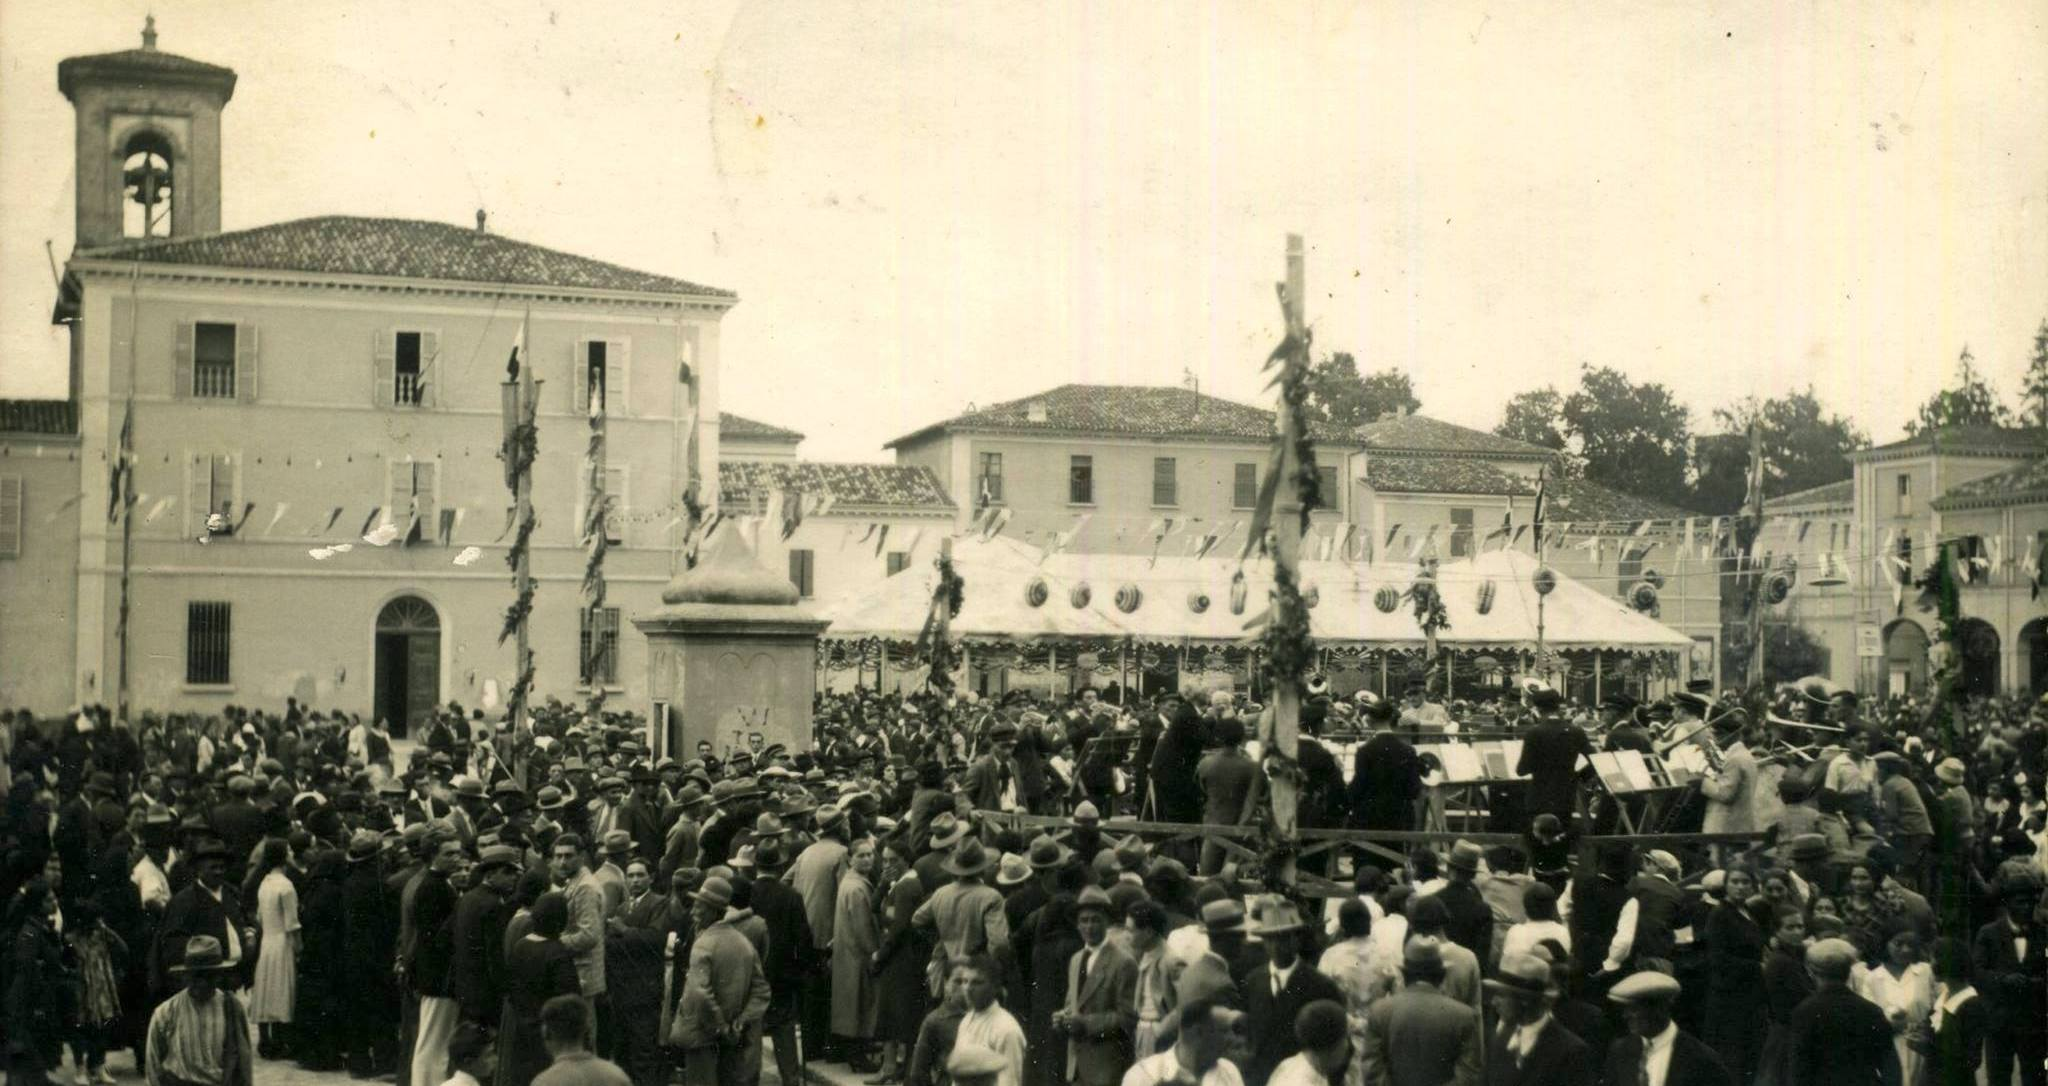
\includegraphics[width=\textwidth]{festa1}
    \vspace{-0.8cm}
\end{figure}

\begin{figure}[htb]
    \centering
    \vspace{-0.45cm}
    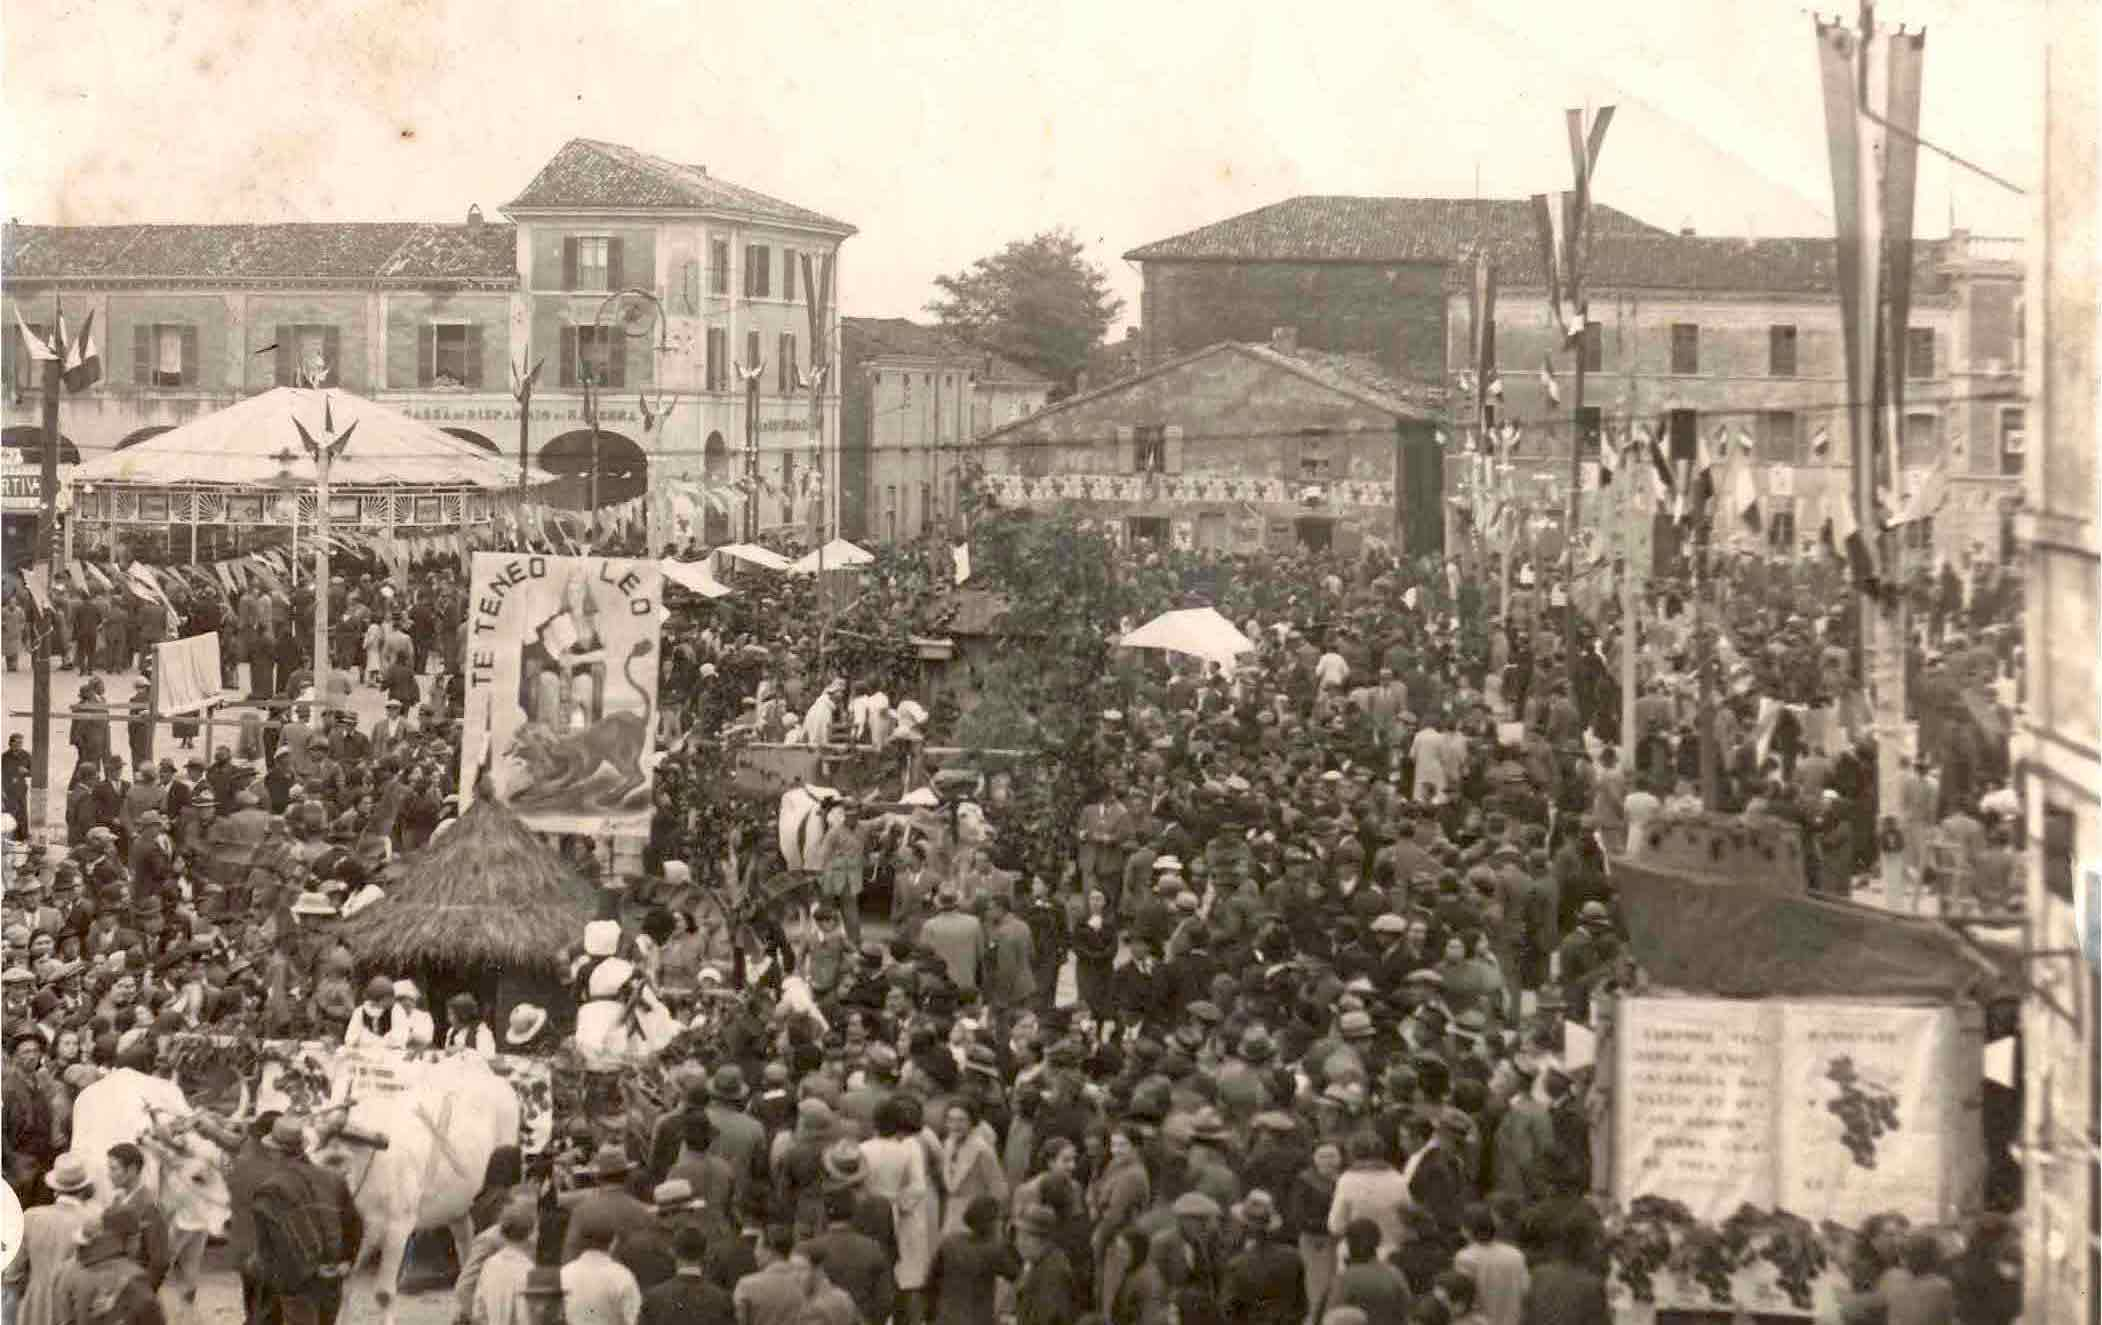
\includegraphics[width=\textwidth]{festa2}
    \caption[Festa dell'uva]{Piazza Monti durante la festa dell'uva 1936. La festa descritta nella storiella probabilmente è la `Festa Gròsa', più antica rispetto alla festa dell'uva. \label{fig:festa2}}
    \vspace{-0.8cm}
\end{figure}
